\subsubsection{Шаговый модуль}

Шаговый модуль является интерфейсом переключения фаз шагового двигателя и
обладает только одним доступным другим модулям методом - методом включения
следующего (или предыдущего, в зависимости от желаемого направления движения)
алгоритмического шага управления двигателем (см. \ref{sec_step_control_algos}
о циклической природе алгоритмических шагов), фактически управляя только
полярностью напряжения, подаваемого на фазы. Модуль может работать в одном из трёх
алгоритмов переключения обмоток - однофазном, двухфазном или полуфазном.

Такая структура позволяет полностью изолировать более высокоуровневые модули от
того, как реализуются шаги двигателя, какой алгоритм переключения фаз
используется и т.д., оставляя при этом другим модулям ответственность о таких вещах
как поддержание требуемых токов и т.п.

\subsubsection{Модуль ОС по положению}

Как было показано в разделе \ref{sec_feedback_control}, эффективность управления
можно повысить, если переключать фазы двигателя исходя из величины оптимальногого
при данных условиях угла коммутации. Алгоритм определения оптимального угла
коммутации описывается в разделе \ref{sec_comm_angle}.

Покажем принцип переключения активной фазы шагового двигателя на примере простого
четырёхфазного шагового двигателя. Условно процесс движения ротора шагового двигателя
можно разделить на элементарные части, состоящие из двух этапов при нормальной
работе и третьего этапа выпада из синхронизма:

\begin{enumerate}
    \item Этап движения
    \item Этап переключения
    \item Этап выпада из сихронизма
\end{enumerate}

Каждый из этих этапов имеет место в тот момент, когда ротор находится в
соответствующей зоне рассогласования векторов магнитных полей статора и ротора
(пренебрежём на данном этапе конечной скоростью нарастания тока в фазах, описанным
в разделе \ref{sec_feedback_control}).

Таким образом, решение о необходимости переключения фаз принимается на основании
анализа того, в какой зоне находится ротор двигателя в данный момент. Найдём условия,
необходимые для этого, проанализировав процесс вращения ротора двигателя в
положительном и отрицательном направлениях.

\textit{Зоной движения} будем называть зону, в которой ротор совершает движения в рамках
текущего шага, включена нужная фаза и, следовательно, перелюкчение не требуется.

\textit{Зоной переключения} будем называть зону, в которой пришло время включения
следующей фазы. Зафиксировав, что ротор находится в этой зоне, модуль ОС по положению
даёт команду шаговому модулю сделать один шаг в направлении движения.

\textit{Зоной выпада из синхронизма} будем называть зону, в которую попадает ротор
двигателя в случае пропуска шагов или возникновения некоторой непредвиденной ситуации
(например, удара, отбросившего ротор назад). Так как зоны не пересекаются, но граничат
друг с другом, зону выпада из синхронизма можно определить как всю область вне зон
движения и переключения.

В соответствие с принятыми обозначениями, будем обозначать угловое положение
ротора (угловое положение вектора магнитного поля ротора) как $\theta$.
Угловое положение вектора магнитного поля статора обозначим $\phi_\textit{акт}$.

\paragraph{Зоны движения и переключения}
\subparagraph{Движение в положительном направлении}
\begin{figure}
    \centering
    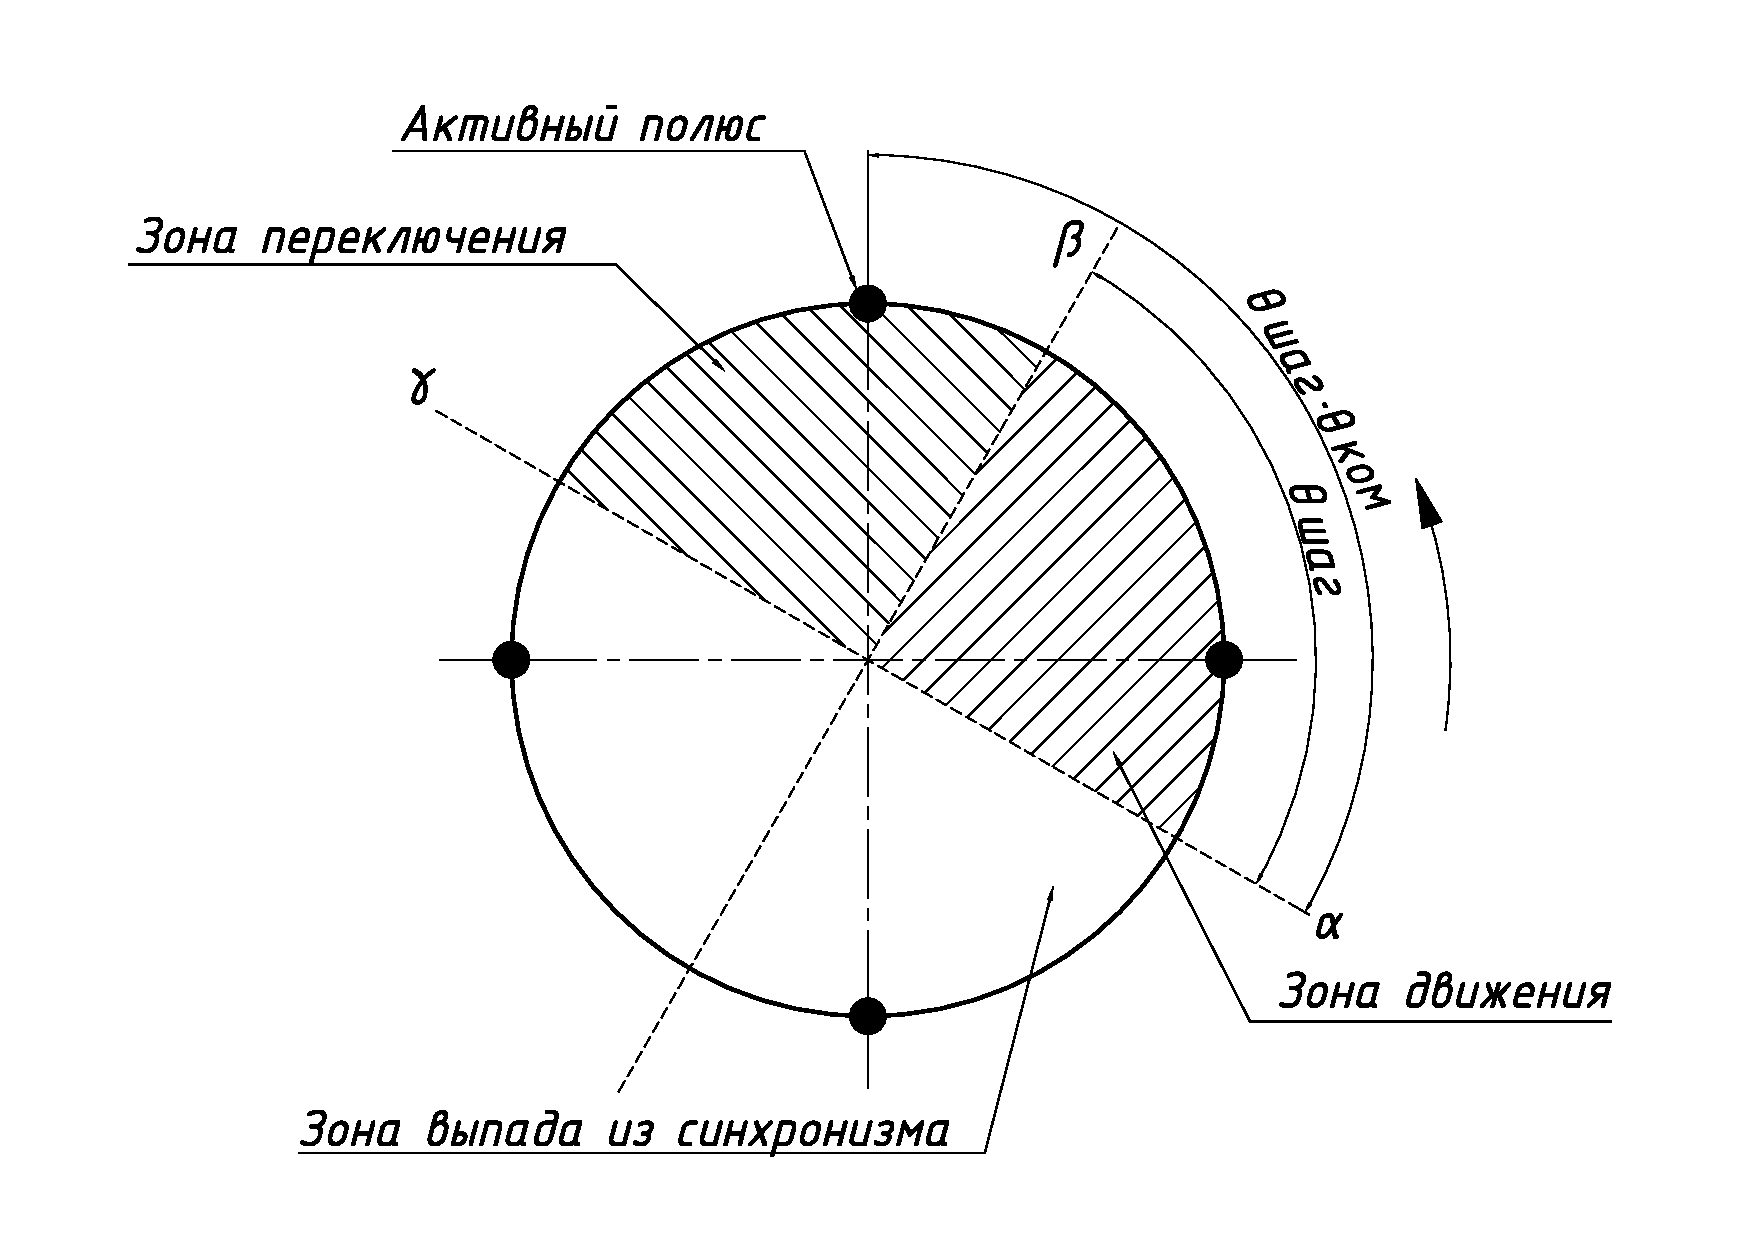
\includegraphics[width=0.7\textwidth, keepaspectratio]
                    {./src/pictures/feedback_control/pole_switch_zones_with_positive_dir}
    \caption{Зоны рассогласований магнитных векторов ротора и статора при вращении в положительном направлении}
    \label{pole_switch_zones_with_positive_dir}
\end{figure}

В зоне движения угловое положение ротора $\theta$ будет удовлетворять следующему условию:

\begin{equation}
    \label{movement_zone_posit_dir_for_curr_pos}
    \begin{array}{ccccc}
        \alpha & \leq & \theta & < & \beta                                         \\
        \phi_\textit{акт} - \theta_\textit{ком}
        & \leq  & \theta
        & <     &\phi_\textit{акт} - (\theta_\textit{ком} - \theta_\textit{шаг})
    \end{array}
\end{equation}

Преобразовав это неравенство, получим выражение, описывающее границы зоны движения
в величинах рассогласования векторов магнитных полей статора и ротора:

\begin{equation}
    \label{movement_zone_posit_dir_for_delta}
    \theta_\textit{ком} - \theta_\textit{шаг}
    < \phi_\textit{акт} - \theta
    \leq \theta_\textit{ком}
\end{equation}

В зоне переключения угловое положение ротора $\theta$ будет удовлетворять следующему условию:

\begin{equation}
    \label{switch_zone_posit_dir_for_curr_pos}
    \begin{array}{ccccc}
        \beta & \leq & \theta & < & \gamma                                         \\
        \phi_\textit{акт} - (\theta_\textit{ком} - \theta_\textit{шаг})
        & \leq  & \theta
        & <     &\phi_\textit{акт} - (\theta_\textit{ком} - 2\theta_\textit{шаг})
    \end{array}
\end{equation}

Преобразовав это неравенство, получим выражение, описывающее границы зоны переключения
в величинах рассогласования векторов магнитных полей статора и ротора:

\begin{equation}
    \label{switch_zone_posit_dir_for_delta}
    \theta_\textit{ком} - 2\theta_\textit{шаг}
    < \phi_\textit{акт} - \theta
    \leq \theta_\textit{ком} - \theta_\textit{шаг}
\end{equation}


\subparagraph{Движение в отрицательном направлении}
\begin{figure}
    \centering
    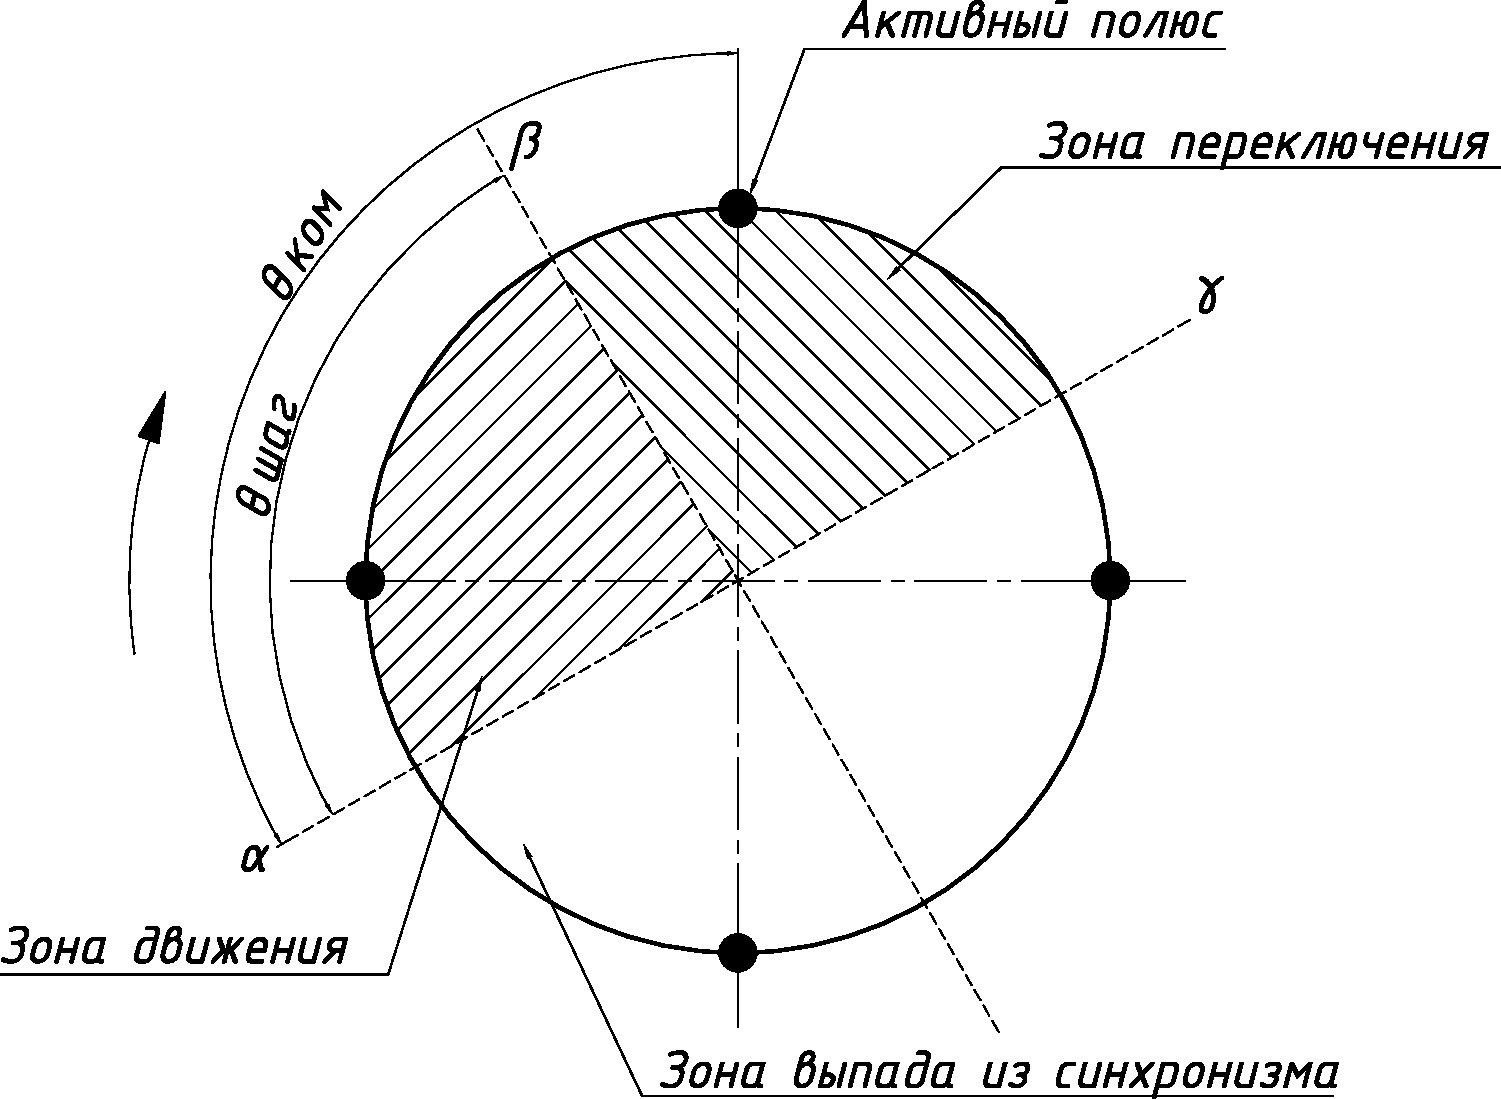
\includegraphics[width=0.7\textwidth, keepaspectratio]
                    {./src/pictures/feedback_control/pole_switch_zones_with_negative_dir}
    \caption{Зоны рассогласований магнитных векторов ротора и статора при вращении в отрицательном направлении}
    \label{pole_switch_zones_with_negative_dir}
\end{figure}

В зоне движения угловое положение ротора $\theta$ будет удовлетворять следующему условию:

\begin{equation}
    \label{movement_zone_negat_dir_for_curr_pos}
    \begin{array}{ccccc}
        \beta & < & \theta & \leq & \alpha                                         \\
        \phi_\textit{акт} + \theta_\textit{ком} - \theta_\textit{шаг}
        & <     & \theta
        & \leq  &\phi_\textit{акт} + \theta_\textit{ком}
    \end{array}
\end{equation}

Преобразовав это неравенство, получим выражение, описывающее границы зоны движения
в величинах рассогласования векторов магнитных полей статора и ротора:

\begin{equation}
    \label{movement_zone_negat_dir_for_delta}
    -\theta_\textit{ком}
    \leq \phi_\textit{акт} - \theta
    < \theta_\textit{шаг} - \theta_\textit{ком}
\end{equation}

В зоне переключения угловое положение ротора $\theta$ будет удовлетворять следующему условию:

\begin{equation}
    \label{switch_zone_negat_dir_for_curr_pos}
    \begin{array}{ccccc}
        \gamma & < & \theta & \leq & \beta                                         \\
        \phi_\textit{акт} + \theta_\textit{ком} - 2\theta_\textit{шаг}
        & <     & \theta
        & \leq  & \phi_\textit{акт} + \theta_\textit{ком} - \theta_\textit{шаг}
    \end{array}
\end{equation}

Преобразовав это неравенство, получим выражение, описывающее границы зоны переключения
в величинах рассогласования векторов магнитных полей статора и ротора:

\begin{equation}
    \label{switch_zone_negat_dir_for_delta}
    \theta_\textit{шаг} - \theta_\textit{ком}
    \leq \phi_\textit{акт} - \theta
    < 2\theta_\textit{шаг} - \theta_\textit{ком}
\end{equation}


\subparagraph{Обобщение результатов}

Обозначив направление движения как $\textit{dir} = \pm 1$ и объединив формулы
для двух направлений движений, получим из (\ref{movement_zone_posit_dir_for_delta})
и (\ref{movement_zone_negat_dir_for_delta}) для зоны движения

\begin{equation}
    \label{movement_zone_for_delta}
    \theta_\textit{ком} - \theta_\textit{шаг}
    < dir \cdot (\phi_\textit{акт} - \theta)
    \leq \theta_\textit{ком}
\end{equation}

и из (\ref{switch_zone_posit_dir_for_delta})
и (\ref{switch_zone_negat_dir_for_delta}) для зоны переключения

\begin{equation}
    \label{switch_zone_for_delta}
    \theta_\textit{ком} - 2\theta_\textit{шаг}
    < dir \cdot (\phi_\textit{акт} - \theta)
    \leq \theta_\textit{ком} - \theta_\textit{шаг}
\end{equation}

\paragraph{Зона выпада из синхронизма}

При попадании в зону выпада из синхронизма, не зависимо от причин приведших к этому,
модуль обратной связи по положению должен восстановить информацию о том,
в зоне переключения какой фазы ротор находится в данный момент. Полагаем, что для
продолжения движения в нужном направлении, необходимо, чтобы шаговый модуль
шаг в нужном направлении. Для этого необходимо обновить информацию о том, на каком
алгоритмическом шаге ротор двигателя находится в данный момент
(см. \ref{sec_step_control_algos} о циклической природе алгоритмических шагов).

Полагаем, что ротор находится в зоне переключения некоторой <<мнимо~--~активной>> фазы,
тогда информация об угловом положении вектора магнитного поля, которое бы имело место,
если бы фаза была действительно включена, позволит обновить информацию о текущем
алгоритмическом шаге шагового модуля. Это позволит шаговому модулю при получении
команды движения в заданном направлении запитать нужную фазу, сделав корректный
алгоритмический шаг.

Определеним формулы для вычисления углового вектора магнитного положения
<<мнимо~--~активной>> фазы для разных направлений движения.

\subparagraph{Положительное направление движения}

Из формулы (\ref{switch_zone_posit_dir_for_curr_pos}) получим

\begin{equation}
    \label{sync_restore_posit_dir_active_pole_pos_conditions}
    \phi_\textit{акт}
    \leq \theta + \theta_\textit{ком} - \theta_\textit{шаг}
    < \phi_\textit{акт} + \theta_\textit{шаг}
\end{equation}

Пусть $T = \theta + \theta_\textit{ком} - \theta_\textit{шаг}$, тогда

\begin{equation}
    \label{sync_restore_posit_dir_active_pole_pos}
    \phi_\textit{акт} = T - mod(T, \theta_\textit{шаг})
\end{equation}
где $mod$ - операция вычисления остатка от деления с сохранением знака делимого.

\subparagraph{Отрицательное направление движения}
Из формулы (\ref{switch_zone_negat_dir_for_curr_pos}) получим

\begin{equation}
    \label{sync_restore_negat_dir_active_pole_pos_conditions}
    \phi_\textit{акт} - \theta_\textit{шаг}
    < \theta - \theta_\textit{ком} + \theta_\textit{шаг}
    \leq \phi_\textit{акт}
\end{equation}

Пусть $D = \theta - \theta_\textit{ком} + \theta_\textit{шаг}$, тогда

\begin{equation}
    \label{sync_restore_negat_dir_active_pole_pos}
    \phi_\textit{акт} =
        \begin{cases}
            D,                                                      & \mbox{если } D - mod(D, \theta_\textit{шаг}) = 0 \\
            D - mod(D, \theta_\textit{шаг}) + \theta_\textit{шаг},  & \mbox{если } D - mod(D, \theta_\textit{шаг}) \ne 0)
        \end{cases}
\end{equation}
где $mod$ - операция вычисления остатка от деления с сохранением знака делимого.
